\documentclass[12pt, a5paper]{article}

\usepackage[top=1cm,bottom=1cm]{geometry}
\usepackage[utf8]{inputenc}
\usepackage{amssymb, amsmath, amsbsy}
\usepackage{mathpazo}
\usepackage{tikz}
\renewcommand{\familydefault}{\sfdefault}

\begin{document}
\subsection*{Lattice Multiplication}
\begin{center}
	\begin{tabular}{cccc}
	\empty & \empty & 2 & 8 \\
	\empty & $\times$ & 4 & 7 \\
	\hline
	1 & 3 & 1 & 6
	\end{tabular}
\end{center}

	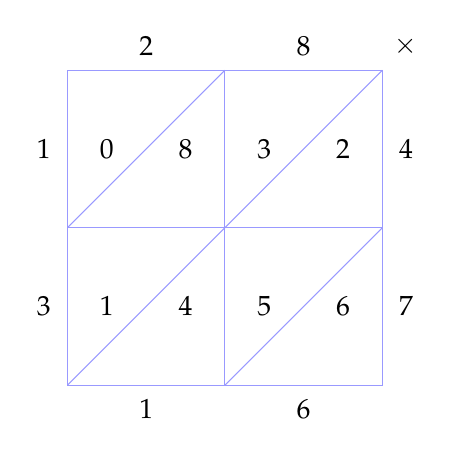
\begin{tikzpicture}
	\draw[draw=blue!40] (0,0) rectangle (2,2);
	\draw[draw=blue!40] (2,2) rectangle (4,4);
	\draw[draw=blue!40] (2,0) rectangle (4,2);
	\draw[draw=blue!40] (0,2) rectangle (2,4);
	% diagonals
	\draw[draw=blue!40] (0,0) -- (2,2);
	\draw[draw=blue!40] (0,2) -- (2,4);
	\draw[draw=blue!40] (2,0) -- (4,2);
	\draw[draw=blue!40] (2,2) -- (4,4);
	% numbers
	\draw (1, 4.3) node {$2$};
	\draw (3, 4.3) node {$8$};
	
	\draw (4.3, 3) node {$4$};
	\draw (4.3, 1) node {$7$};
	% numbers PRODUCT
	\draw (1, -.3) node {$1$};
	\draw (3, -.3) node {$6$};
	
	\draw (-.3, 3) node {$1$};
	\draw (-.3, 1) node {$3$};
	% previous CALCs
	\draw (.5, 1) node {$1$};
	\draw (.5, 3) node {$0$};
	\draw (1.5, 1) node {$4$};
	\draw (1.5, 3) node {$8$};

	\draw (2.5, 1) node {$5$};
	\draw (2.5, 3) node {$3$};
	\draw (3.5, 1) node {$6$};
	\draw (3.5, 3) node {$2$};
	
	\draw (4.3, 4.3) node {$\times$};
	\end{tikzpicture}

\end{document}
